\chapter{Lösungsansatz}
\label{sec:Lösungsansatz}

Die numerische Umsetzung erfolgt in Abaqus/CAE (Standard/Static) und orientiert sich an einem modularen Aufbau (s. \secref{sec:Abaqus .cae-file}), um die Reproduzierbarkeit der Simulation zu gewährleisten. Alle Eingaben wurden unter Berücksichtigung der Einheiten $\mathrm{mm,\ N,\ t,\ s,\ MPa}$ vorgenommen, um die Konsistenz mit den analytischen Berechnungen sicherzustellen. Eingebundene Visualisierungen und in TUM-Moodle eingereichte Ausgaben aus Abaqus sind entsprechend einheitenlos.

Die numerische Untersuchung wird in mehrere Phasen unterteilt, um den Einfluss der Diskretisierungsstrategie und der Elementformulierung auf die Ergebnisgenauigkeit systematisch zu erfassen.

\section{Basismodellierung und initiale Diskretisierung (Teilaufgabe \text{a)})}
\label{sec:Basismodellierung und initiale Diskretisierung}

In der ersten Phase wird die Grundgeometrie der Lochscheibe ohne spezifische Netzoptimierungen abgebildet. Für die Vernetzung wird ein globaler Instanz-Seed von ${2.5}$ gewählt. (\sfigref{fig:lin-unseeded_mesh}) Als Elementtyp kommen lineare Standard-Elemente ohne reduzierte Integration \texttt{CPS4} zum Einsatz. Dieser Ansatz dient als Referenz \texttt{Kuhn\_A2-2\_lin-unseeded.odb}, um die prozentuale Abweichung der Diskretisierung vom analytischen Idealwert zu quantifizieren.

\section{Iterative Netzoptimierung und Sensitivitätsanalyse (Teilaufgabe \text{b)})}
\label{sec:Iterative Netzoptimierung und Sensitivitätsanalyse}

Der Schwerpunkt der Untersuchung liegt auf der schrittweisen Verfeinerung des Modells unter Berücksichtigung einer lizenzbedingten Knotenobergrenze von ${1000}$ nodes. Dieser Prozess wird in drei wesentlichen Veränderungen durchgeführt:
\begin{itemize}
    \item \texttt{Kuhn\_A2-2\_lin-seeded.odb}: Zur Verbesserung der lokalen Auflösung wird ein spezifisches Seeding ohne Bias am Lochrand appliziert. Mittels strukturierter Netzsteuerungen (\texttt{Quad-Structured}) wird eine erste lokale Konzentration der Elemente im Kerbbereich erzielt, während die Elementformulierung zunächst linear beibehalten wird. (\sfigref{fig:lin-seeded_mesh})
    \item \texttt{Kuhn\_A2-2\_quad-seeded\_V1.odb}: In dieser Iteration erfolgt der Wechsel auf quadratische, voll integrierte Elemente \texttt{CPS8}. Da dieser Elementtyp eine höhere Anzahl an Integrationspunkten und Knoten pro Element aufweist, wird die globale Elementanzahl im Vergleich zum linearen Modell reduziert, um die Knotenobergrenze einzuhalten. Um dennoch eine hohe Genauigkeit zu erzielen, wird die Scheibe in Quadranten partitioniert. Dies ermöglicht ein \texttt{Single-Bias Seeding} am Lochrand, welches die Knoten gezielt entlang der erwarteten Spannungsgradienten konzentriert. (\sfigref{fig:quad-seeded_V1_mesh})
    \item \texttt{Kuhn\_A2-2\_quad-seeded\_V2.odb}: Zur Untersuchung der numerischen Stabilität wird eine Sensitivitätsanalyse der Steuerungsparameter durchgeführt. Hierbei wird das Verhältnis zwischen kleinster und größter Elementdistanz (Bias-Ratio) an den radialen Partitionierungen der Quadranten sowie der Außenkanten eingestellt, um die Grenzen der Konvergenz und den Einfluss der Elementverzerrung auf die Spannungsspitzen zu evaluieren. (\sfigref{fig:quad-seeded_V2_mesh})
\end{itemize}

\begin{figure}[htbp]
    \centering

    \begin{subfigure}{0.48\textwidth}
        \centering
        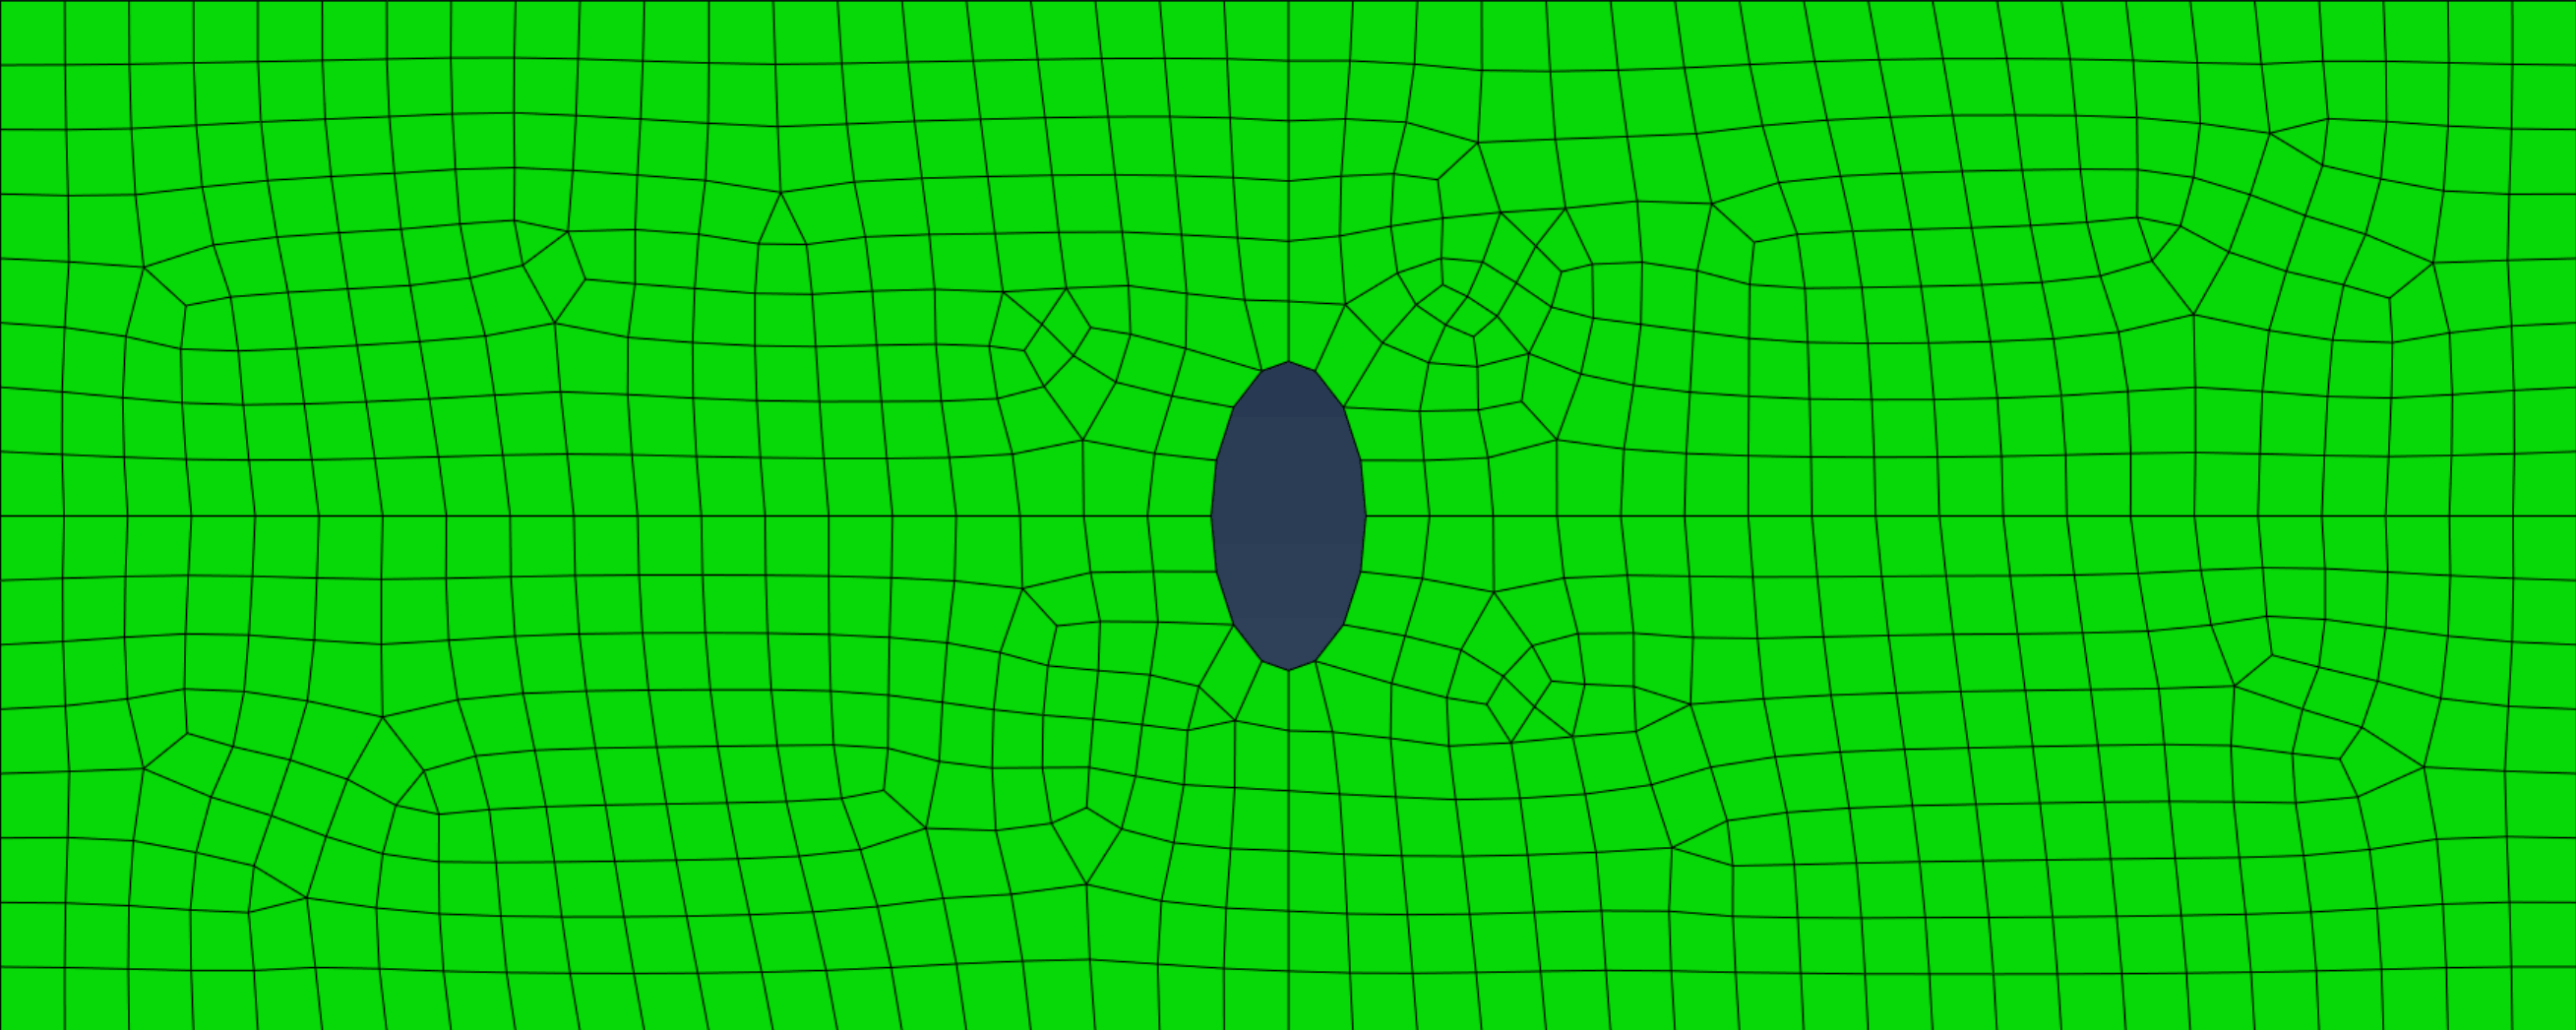
\includegraphics[width=\textwidth]{_ltx/Kuhn_A2-2_lin-unseeded_mesh.png} % Datei für unseeded mesh
        \caption{Mesh der Scheibe mit linearen Elementen und ungesteuertem Seeding}
        \label{fig:lin-unseeded_mesh}
    \end{subfigure}
    \hfill % Schiebt die Bilder auseinander, damit sie nebeneinander stehen
    %\vspace{.5em} % Optional: Zusätzlicher vertikaler Abstand zwischen den Bildern
    \begin{subfigure}{0.48\textwidth}
        \centering
        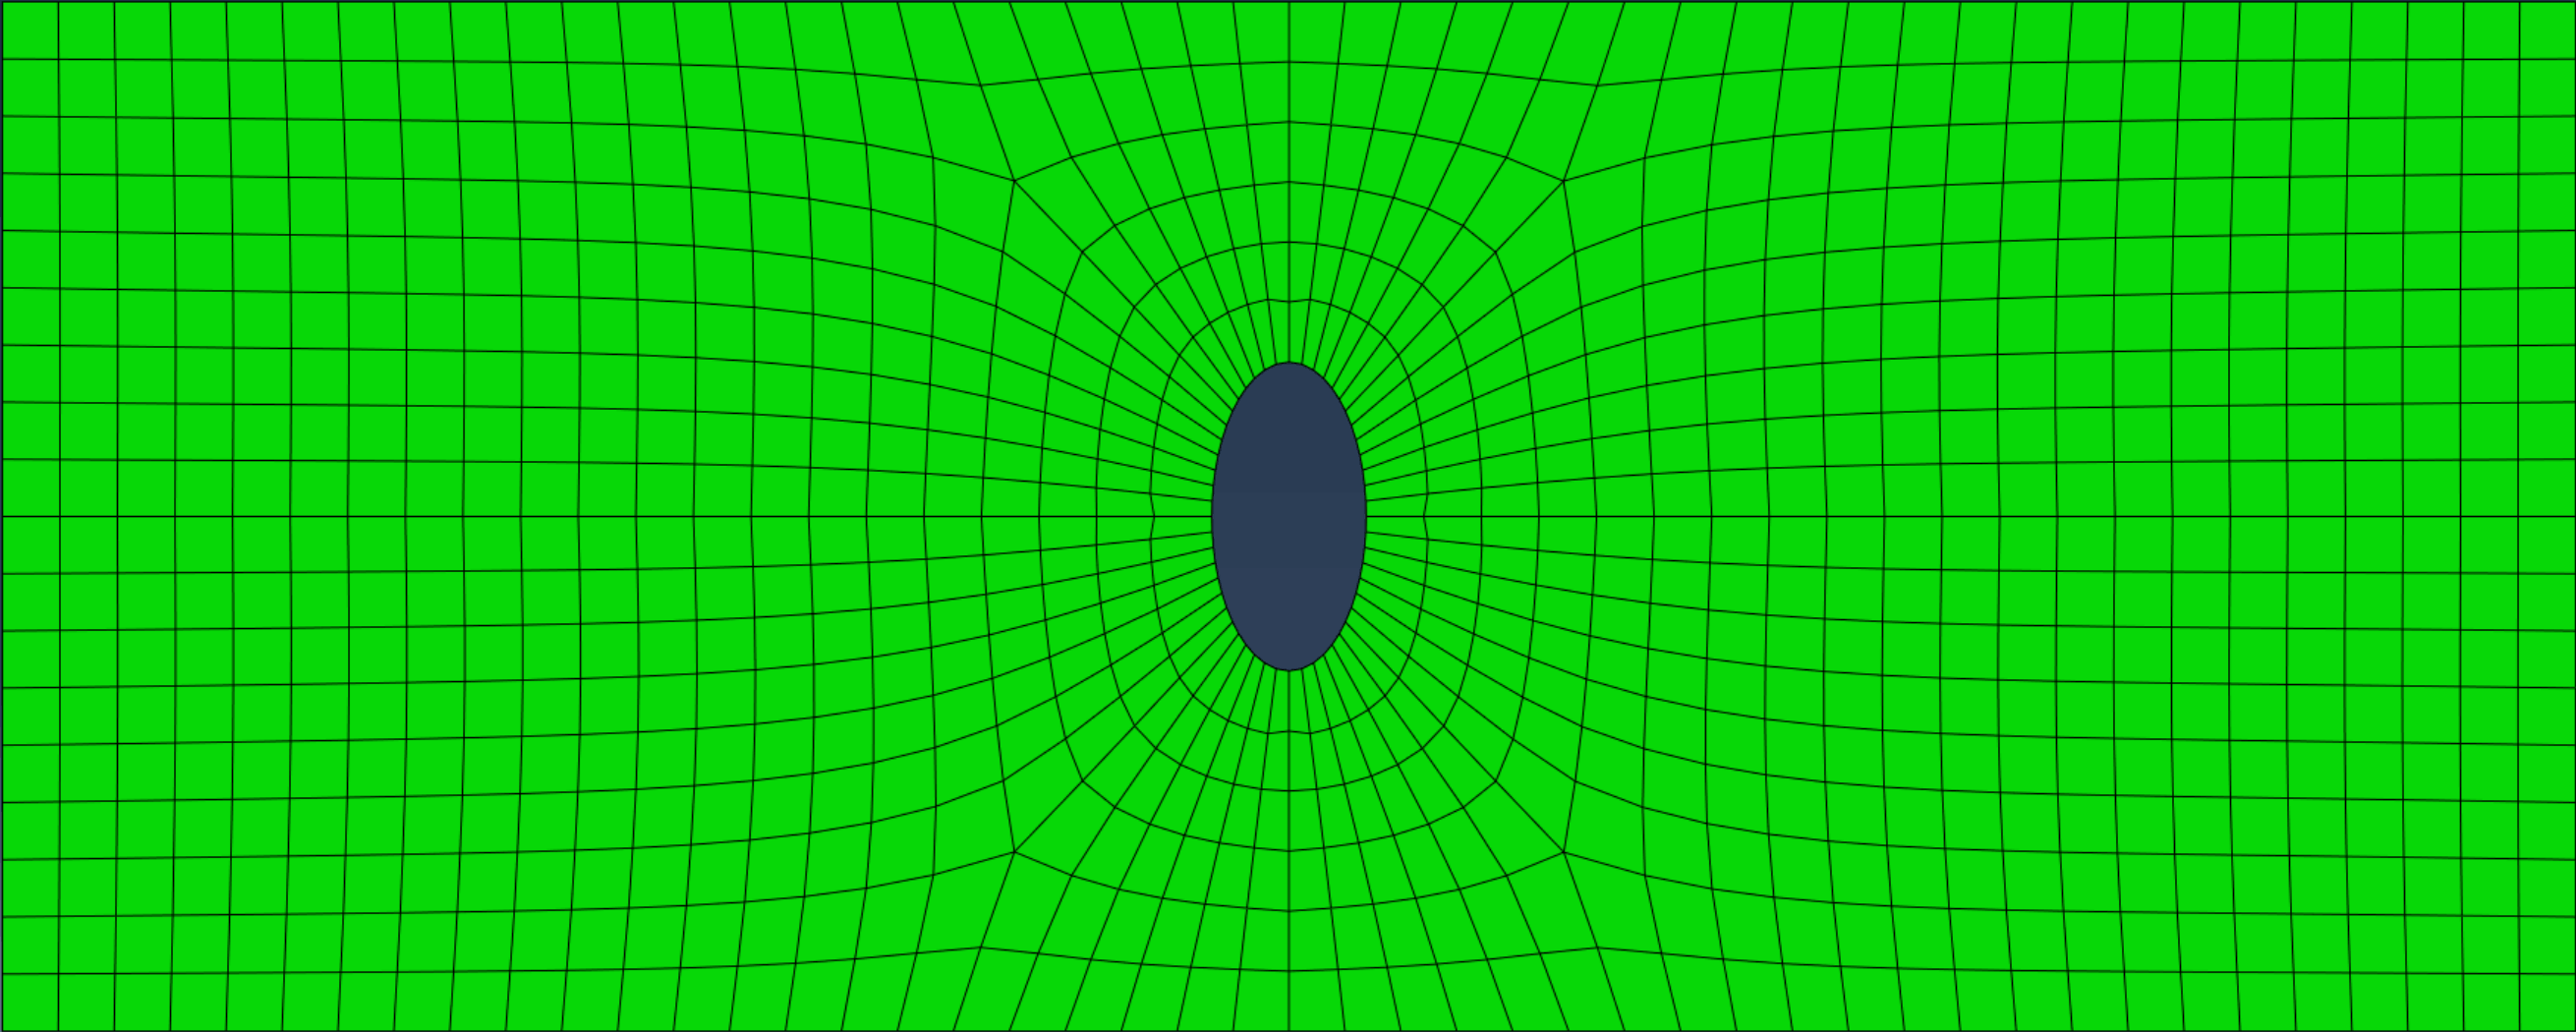
\includegraphics[width=\textwidth]{_ltx/Kuhn_A2-2_lin-seeded_mesh.png} % Datei für seeded mesh
        \caption{Mesh der Scheibe mit linearen Elementen und gesteuertem Seeding}
        \label{fig:lin-seeded_mesh}
    \end{subfigure}

    \vspace{.5em} % Optional: Zusätzlicher vertikaler Abstand zwischen den Bildern

    \begin{subfigure}{0.48\textwidth}
        \centering
        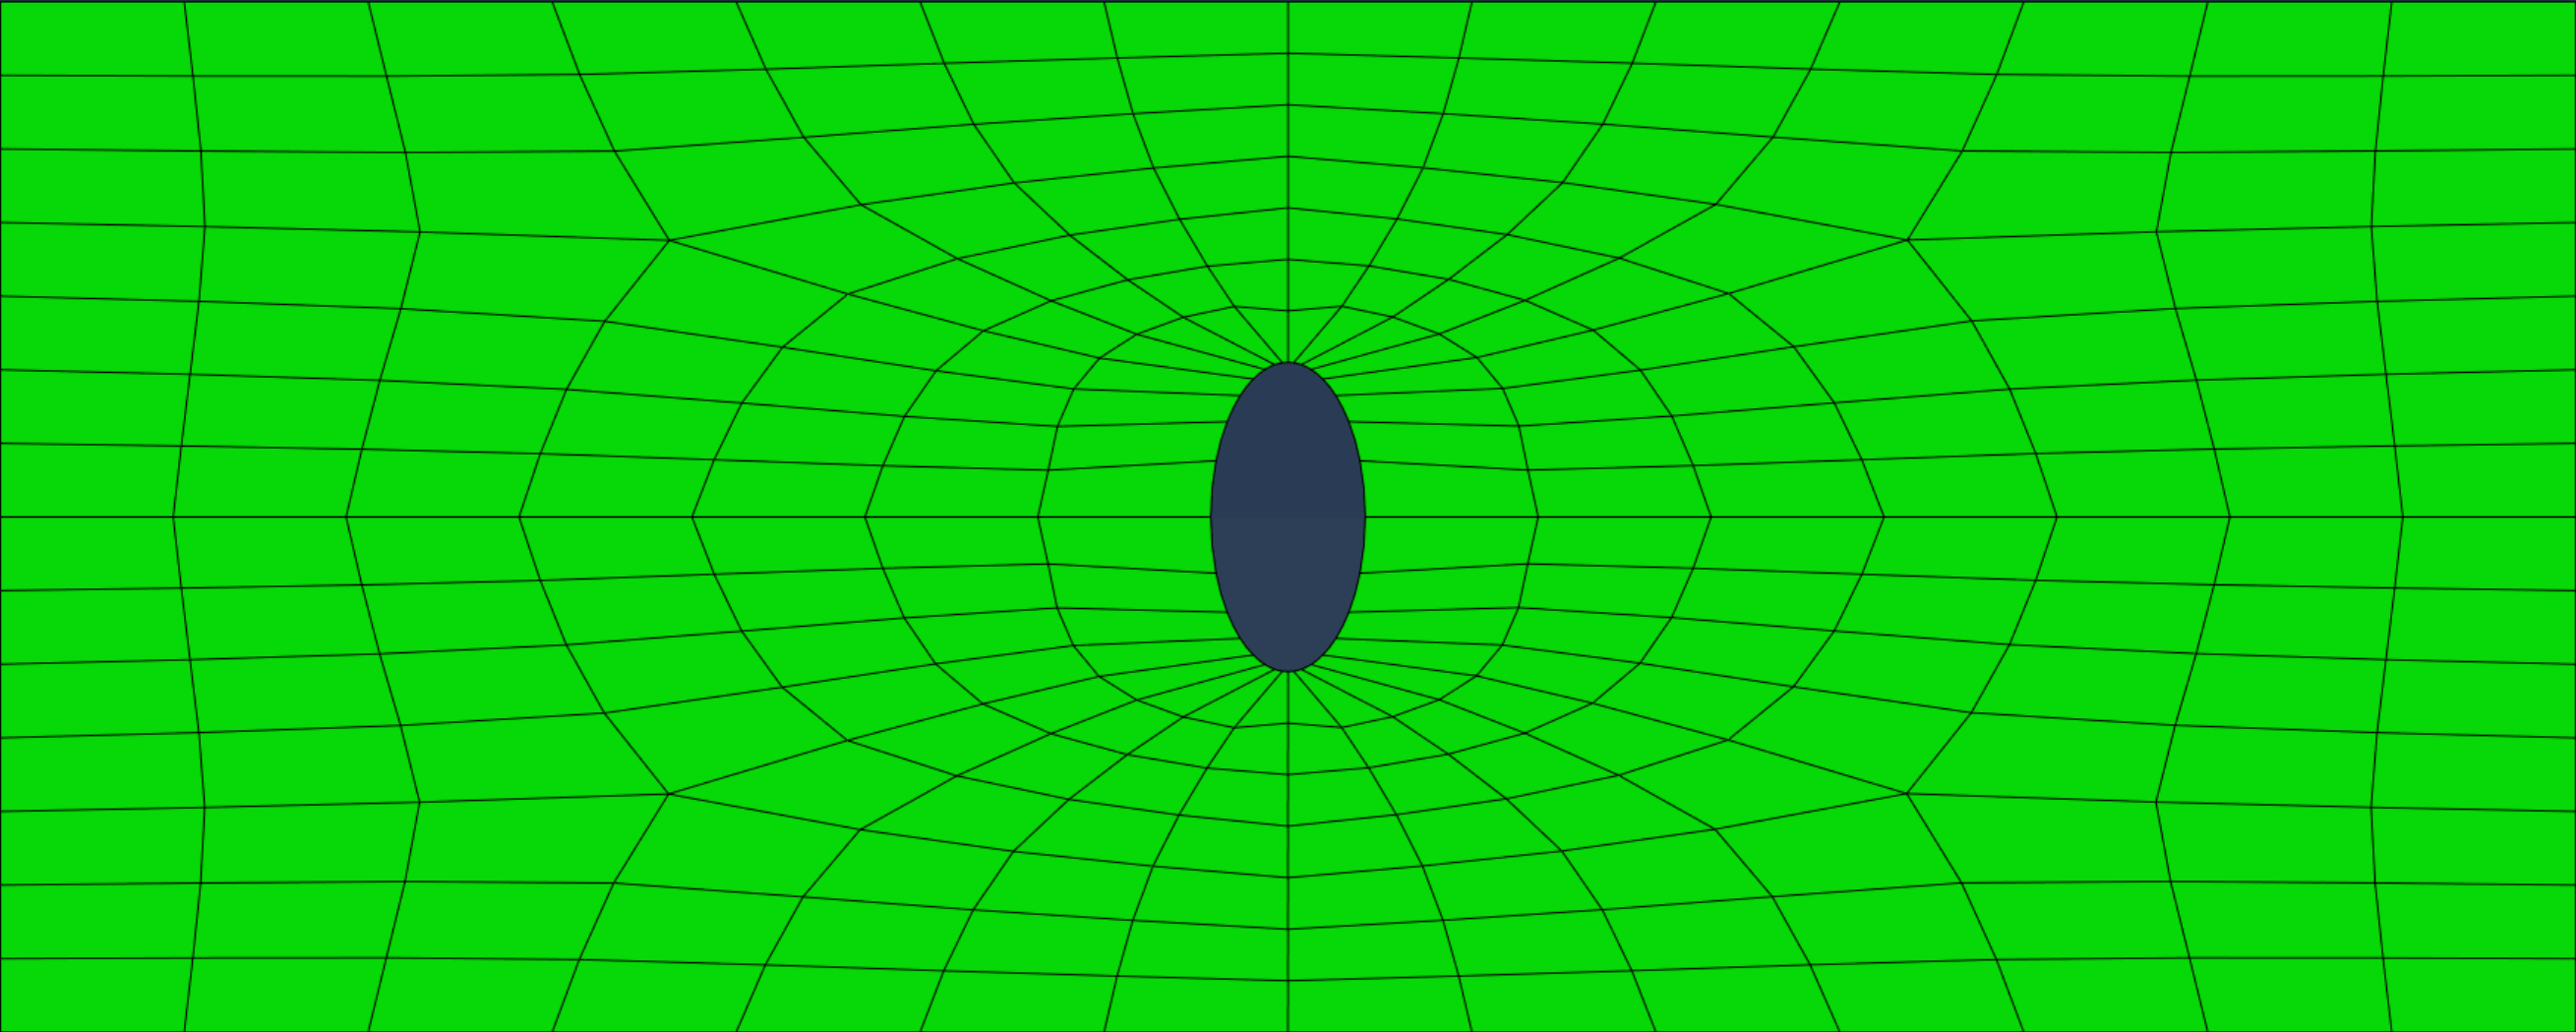
\includegraphics[width=\textwidth]{_ltx/Kuhn_A2-2_quad-seeded_V1_mesh.png} % Datei für quad seeded mesh V1
        \caption{Mesh der Scheibe mit quadratischen Elementen und gesteuertem Seeding V1}
        \label{fig:quad-seeded_V1_mesh}
    \end{subfigure}
    \hfill % Schiebt die Bilder auseinander, damit sie nebeneinander stehen
    %\vspace{.5em} % Optional: Zusätzlicher vertikaler Abstand zwischen den Bildern
    \begin{subfigure}{0.48\textwidth}
        \centering
        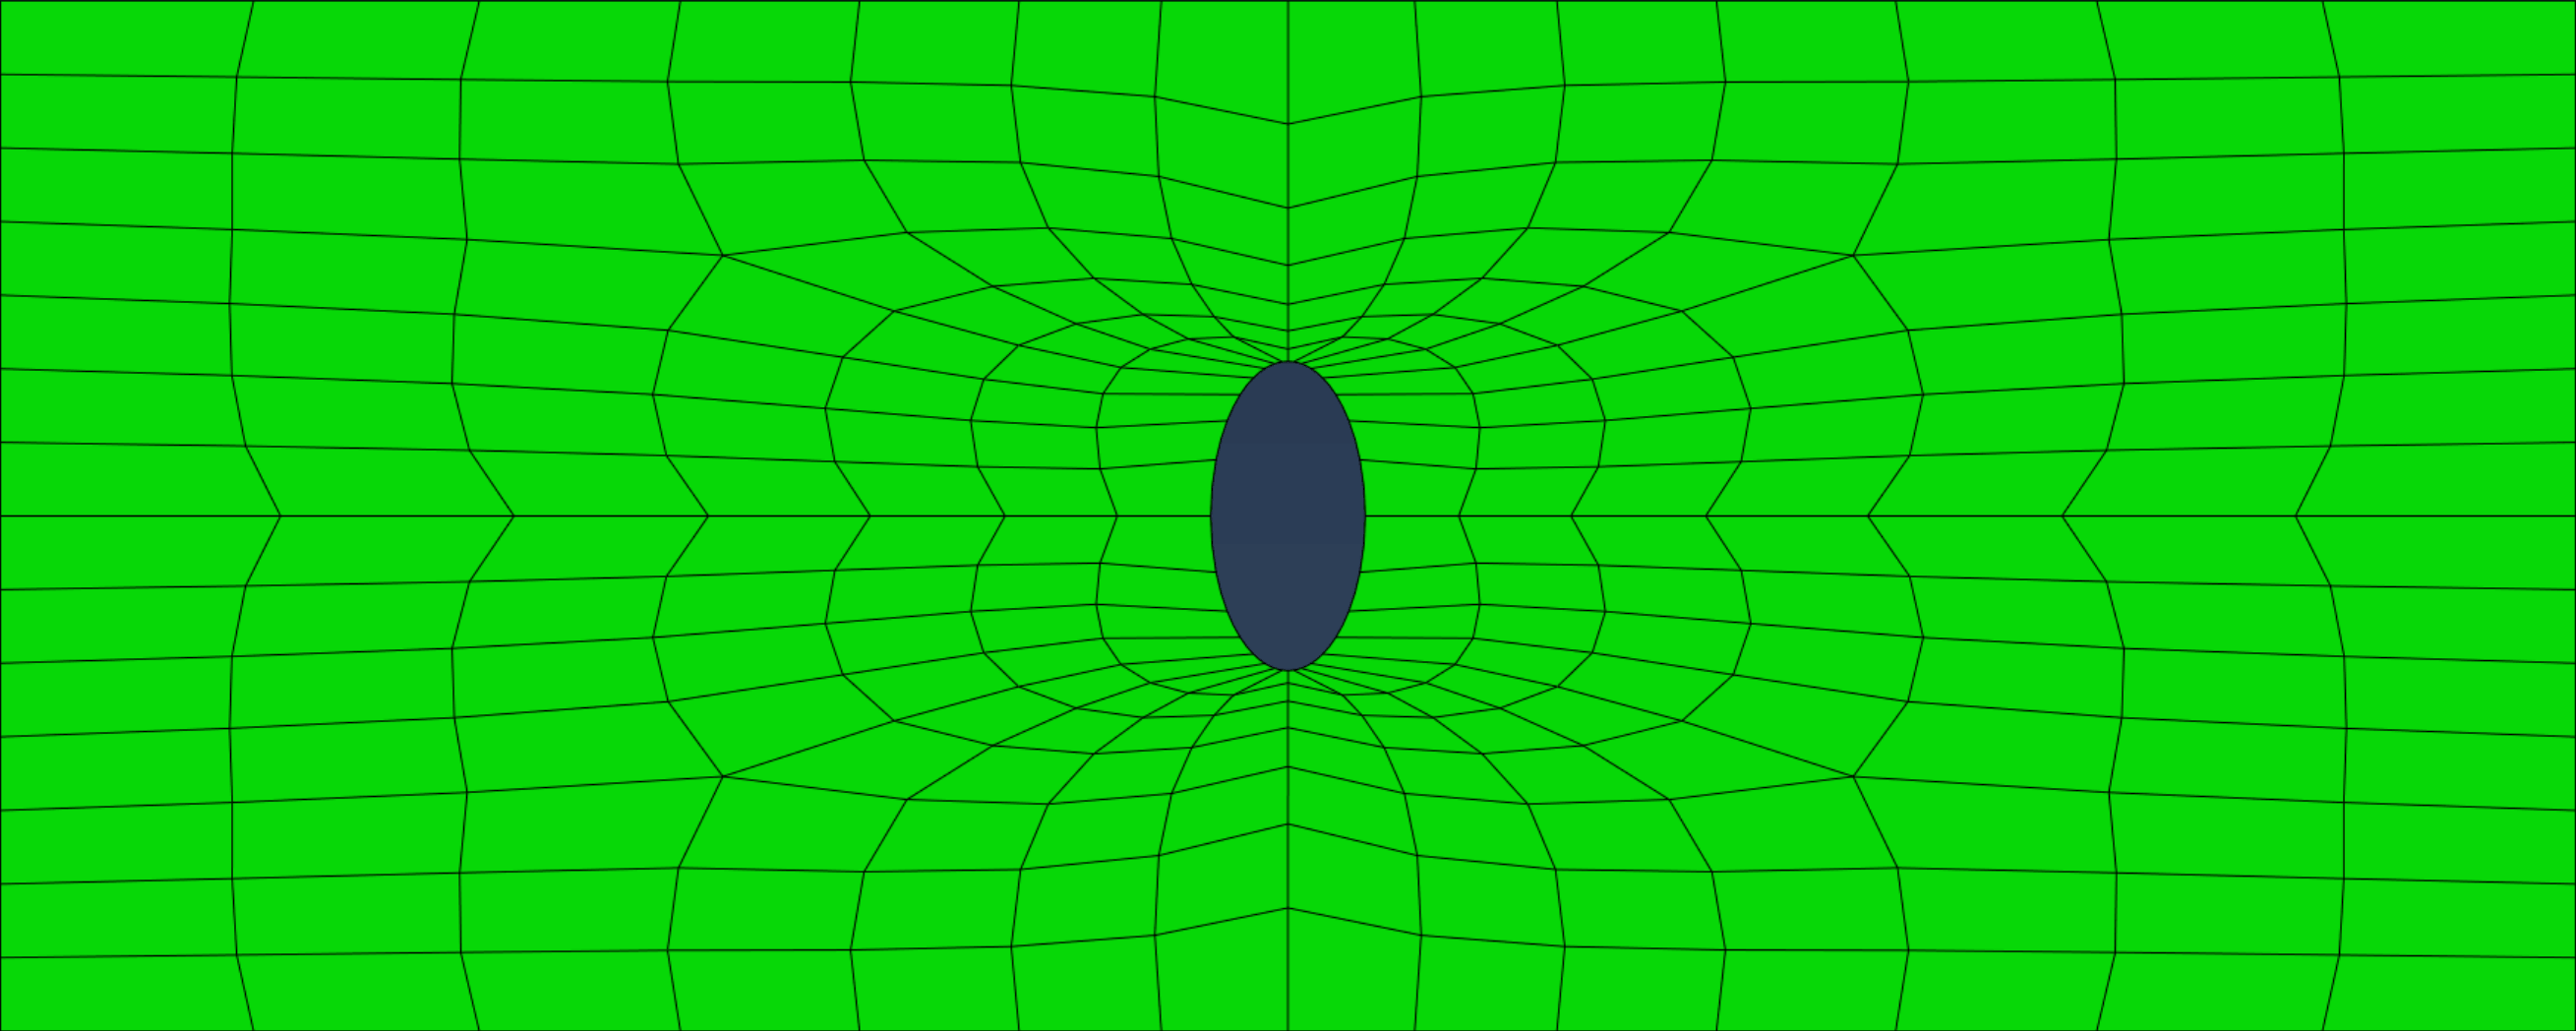
\includegraphics[width=\textwidth]{_ltx/Kuhn_A2-2_quad-seeded_V2_mesh.png} % Datei für quad seeded mesh V2
        \caption{Mesh der Scheibe mit quadratischen Elementen und gesteuertem Seeding V2}
        \label{fig:quad-seeded_V2_mesh}
    \end{subfigure}

    \caption{Mesh der Lochscheibe in den verschiedenen Iterationen der Netzoptimierung}
    \label{fig:Mesh Lochscheibe}
\end{figure}

\section{Pfaddefinition (Teilaufgabe \text{c)})}
\label{sec:Pfaddefinition}

Für die detaillierte Analyse des Spannungsverlaufs über die Scheibenhöhe wird ein vertikaler Auswertungspfad (Pfad $A-A$) definiert. Dieser Pfad liegt bei ${x = 50}$ über die gesamte Höhe der Scheibe. Entlang dieses Pfads werden die Normalspannungen ${\sigma_{xx}}$ extrahiert, um den Gradientenabbau ausgehend von der Kerbe in den ungestörten Bereich der Scheibe grafisch darzustellen und zu diskutieren.